\section{Linearization: Tangent Planes and Differentials} \label{S:10.4.Linearization}

\vspace*{-14 pt}
\framebox{\hspace*{3 pt}
\parbox{6.25 in}{\begin{goals}
  \item What does it mean for a function of two variables to be
    locally linear at a point?
  \item How do we find the equation of the plane tangent to a locally
    linear function at a point?
  \item What does it mean to say that a multivariable function is \emph{differentiable}?
  \item What is the differential of a multivariable function of two
    variables and what are its uses?
\end{goals}} \hspace*{3 pt}}

\subsection*{Introduction}

One of the central concepts in single variable calculus is that the
graph of a differentiable function, when viewed on a very small scale, looks like a
line.  We call this line the tangent line and measure its slope with
the derivative.  In this section, we will extend this concept to
functions of several variables.

Let's see what happens when we look
at the graph of a two-variable function on a small scale.  To begin, let's consider the function
$$ 
f(x,y) = 6 - \frac{x^2}2 - y^2,
$$
whose graph is shown in Figure \ref{F:10.4.tangent.1}.

\begin{figure}[ht]
  \begin{center}
    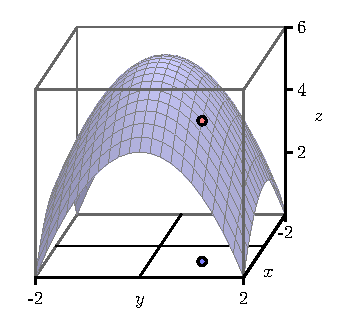
\includegraphics{figures/fig_10_4_tangent_1.eps}
  \end{center}
  \caption{The graph of $f(x,y)=6-x^2/2 - y^2$.}
  \label{F:10.4.tangent.1}
\end{figure}

We choose to study the behavior of this function near the point $(x_0,
y_0) = (1,1)$.  In particular, we wish to view the graph on an
increasingly small scale around this point, as shown in the two plots in Figure
\ref{F:10.4.tangent.2}

\begin{figure}[ht]
  \begin{center}
    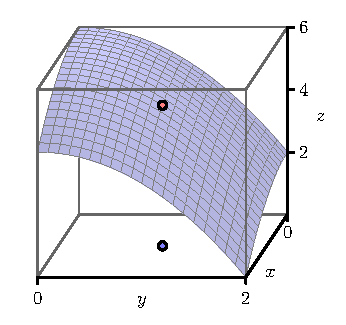
\includegraphics{figures/fig_10_4_tangent_2.eps} \hspace*{20pt}
    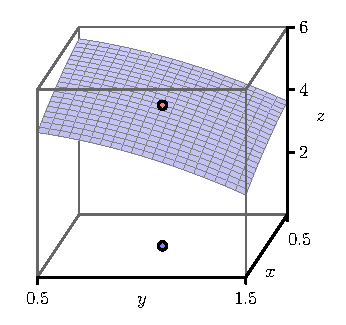
\includegraphics{figures/fig_10_4_tangent_3.eps}
  \end{center}
  \caption{The graph of $f(x,y)=6-x^2/2 - y^2$.}
  \label{F:10.4.tangent.2}
\end{figure}

Just as the graph of a differentiable single-variable function looks like a line
when viewed on a small scale, we see that the graph of this particular two-variable
function looks like a plane, as seen in Figure \ref{F:10.4.tangent.4}.
In the following preview activity, we explore how to find the equation of this plane.

\begin{figure}[ht]
  \begin{center}
    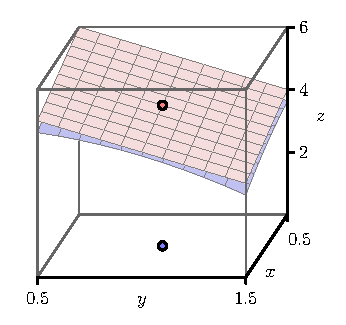
\includegraphics{figures/fig_10_4_tangent_4.eps}
  \end{center}
  \caption{The graph of $f(x,y)=6-x^2/2 - y^2$.}
  \label{F:10.4.tangent.4}
\end{figure}

In what follows, we will also use the important fact\footnote{As we saw in Section \ref{S:9.5.Lines_Planes}, the equation
  of a plane passing through the point $(x_0, y_0, z_0)$ may be written
  in the form $A(x-x_0) + B(y-y_0) + C(z-z_0) = 0$.  If the
  plane is not vertical, then $C\neq 0$, and we can
  rearrange this and hence write
$
    C(z-z_0) = -A(x-x_0) - B(y-y_0) 
$
and thus
\begin{align*}
    z & = z_0-\frac AC(x-x_0) - \frac BC(y-y_0) \\
      & = z_0 + a(x-x_0) + b(y-y_0)
  \end{align*}
  where $a=-A/C$ and $b=-B/C$, respectively.} that the plane passing through $(x_0, y_0, z_0)$ may be expressed in the form
$z = z_0 + a(x-x_0) + b(y-y_0)$, where $a$ and $b$ are constants.

\begin{pa} \label{PA:10.4}  Let $f(x,y) = 6 - \frac{x^2}2 - y^2$, and let $(x_0,y_0)
  = (1,1)$.
\ba
\item Evaluate $f(x,y) = 6 - \frac{x^2}2 - y^2$ and its partial derivatives at $(x_0,y_0)$;  that is, find $f(1,1)$, $f_x(1,1)$, and $f_y(1,1)$.

\item We know one point on the tangent plane;  namely, the $z$-value of the tangent
  plane agrees with the $z$-value on the graph of the function $f(x,y) = 6 - \frac{x^2}2 - y^2$ at the point $(x_0,
  y_0)$.  In other words, both the tangent plane and the graph of the function $f$ contain the point $(x_0, y_0, z_0)$. Use this observation to determine $z_0$ in the expression
  $z = z_0 + a(x-x_0) + b(y-y_0)$.

\item Sketch the traces of the function $f(x,y) = 6 - \frac{x^2}2 - y^2$ for $y=y_0=1$ and $x=x_0=1$
  below in Figure \ref{F:10.4.traces}.  

  \begin{figure}[ht]
    \begin{center}
      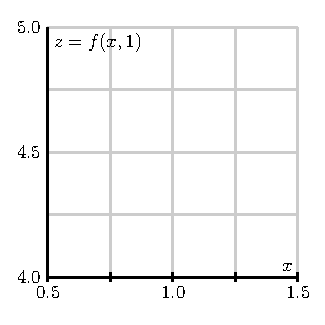
\includegraphics{figures/fig_10_4_tangent_trace_y.eps}
      \hspace*{20pt}
      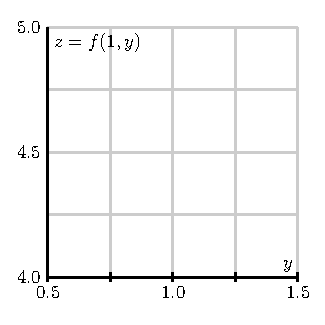
\includegraphics{figures/fig_10_4_tangent_trace_x.eps}
    \end{center}
    \caption{The traces of $f(x,y)$ with $y=y_0=1$ and $x=x_0=1$.}
    \label{F:10.4.traces}
  \end{figure}

\item Determine the equation of the tangent line of the trace that you sketched in the previous part with $y=1$ (in the $x$ direction) at the point $x_0=1$.  

  \begin{figure}[ht]
    \begin{center}
      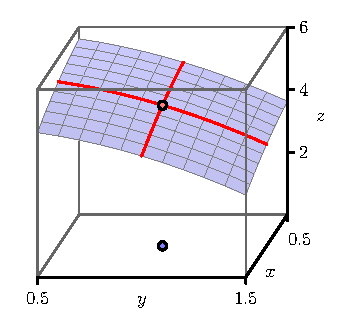
\includegraphics{figures/fig_10_4_tangent_5.eps}
      \hspace*{20pt}
      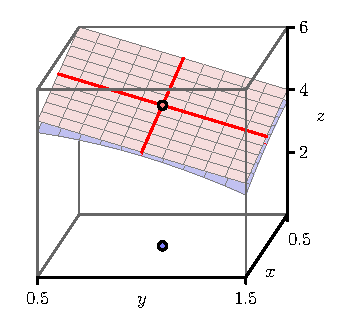
\includegraphics{figures/fig_10_4_tangent_6.eps}
    \end{center}
    \caption{The traces of $f(x,y)$ and the tangent plane.}
    \label{F:10.4.tangent.traces}
  \end{figure}
  
\item Figure \ref{F:10.4.tangent.traces} shows the traces of the
  function and the traces of the tangent plane.  Explain how the
  tangent line of the trace of $f$, whose equation you found in the
  last part of this 
  activity, is related to the tangent plane.  How does this
  observation help you determine the constant $a$ in the equation for the tangent plane $z
  = z_0+a(x-x_0) + b(y-y_0)$?  (Hint: How do you think $f_x(x_0,y_0)$ should be related to $z_x(x_0,y_0)$?)



\item In a similar way to what you did in (d), determine the equation of the tangent line of the
  trace with $x=1$ at the point $y_0=1$.  Explain how this tangent
  line is related to the tangent plane, and use this observation to
  determine the constant $b$ in the equation for the tangent plane
  $z=z_0+a(x-x_0) + b(y-y_0)$. (Hint: How do you think $f_y(x_0,y_0)$ should be related to $z_y(x_0,y_0)$?)

\item Finally, write the equation $z=z_0 + a(x-x_0) + b(y-y_0)$ of the tangent
  plane to the graph of $f(x,y)=6-x^2/2 - y^2$ at the point
  $(x_0,y_0)=(1,1)$. 

\ea

\end{pa}

\begin{activitySolution} 
\ba
\item Since $f_x(x,y) = -x$ and $f_y(x,y) = -2y$ we have $f(1,1) = \frac{9}{2}$, $f_x(1,1) = -1$, and $f_y(1,1) = -2$. 

\item Since $f(1,1) = \frac{9}{2}$ we must have $z_z=\frac{9}{2}$. 

\item 
%The traces in the $x$ and $y$ directions are shown below.  

%  \begin{figure}[ht]
%    \begin{center}
%      \resizebox{!}{2.5in}{\includegraphics{figures/fig_10_4_tangent_trace_x_sol.eps}}
%      \hspace*{20pt}
%      \resizebox{!}{2.5in}{\includegraphics{figures/fig_10_4_tangent_trace_y_sol.eps}}
 %   \end{center}
%    \caption{The traces of $f(x,y)$ with $y=y_0=1$ and $x=x_0=1$.}
%    \label{F:10.4.traces_sol}
%  \end{figure}

\item The slope of the tangent line to the trace of $f$ with $y=1$ (in the $x$ direction) at $x_0=1$ is $f_x(1,1) = -1$. So the equation of this tangent line is $y = \frac{9}{2} - (x-1)$. 


  
\item The tangent line of the trace on the surface in the $x$ direction at the point $(x_0,y_0,z_0)$ is the same as the tangent line found in the 
  last part of this activity with $y$ constant at $1$. The slope of this line tells us how $z$ changes as we change only the $x$ coordinate at this point. So that slope, $f_x(x_0,y_0)$, should be the value of $a$  in the equation $z = z_0+a(x-x_0) + b(y-y_0)$ of the tangent plane. In other words, $f_x(x_0,y_0)$ should be equal to $z_x(x_0,y_0)$. 


\item The slope of the tangent line to the trace of $f$ with $x=1$ (in the $y$ direction) at $y_0=1$ is $f_y(1,1) = -2$. So the equation of this tangent line is $y = \frac{9}{2} - (y-1)$. The tangent line of the trace on the surface in the $y$ direction at the point $(x_0,y_0,z_0)$ is the same as the tangent line $y = \frac{9}{2} - (y-1)$ just found with $x$ constant at $1$. The slope of this line tells us how $z$ changes as we change only the $y$ coordinate at this point. So that slope, $f_y(x_0,y_0)$, should be the value of $b$  in the equation $z = z_0+a(x-x_0) + b(y-y_0)$ of the tangent plane. In other words, $f_y(x_0,y_0)$ should be equal to $z_y(x_0,y_0)$. 

\item The equation of the tangent plane to the graph of $f(x,y)=6-x^2/2 - y^2$ at the point $(x_0,y_0)=(1,1)$ is
\[z=z_0 + a(x-x_0) + b(y-y_0) = z_0 + f_x(x_0,y_0)(x-x_0) + f_y(x_0,y_0)(y-y_0) = \frac{9}{2} - (x-1) - 2(y-1).\]

\ea
\end{activitySolution}

\aftera

%\begin{pa} \label{PA:10.4} 
  As we saw in Section \ref{S:9.5.Lines_Planes}, the equation
  of a plane passing through the point $(x_0, y_0, z_0)$ may be written
  as $A(x-x_0) + B(y-y_0) + C(z-z_0) = 0$.  If the
  plane is not vertical, then $C\neq 0$, and we can
  rearrange this as
  \begin{align*}
    C(z-z_0) & = -A(x-x_0) - B(y-y_0) \\
    z & = z_0-\frac AC(x-x_0) - \frac BC(y-y_0) \\
    z & = z_0 + a(x-x_0) + b(y-y_0)
  \end{align*}
  where we have written the constants $-A/C$ and $-B/C$ as $a$ and
  $b$, respectively.
  
  In this activity, we would like to understand the geometric
  significance of this expression.  We will consider the plane whose
  equation is the graph of the function $f(x,y)$:
  $$
  z = f(x,y) = 3 - \frac12(x-1) - 2(y-1).
  $$
  This plane is shown in Figure \ref{F:10.4.tangent.7}.  On the right,
  we have added the traces through the point $(x_0,y_0) = (1,1)$.
  
  \begin{figure}[ht]
    \begin{center}
      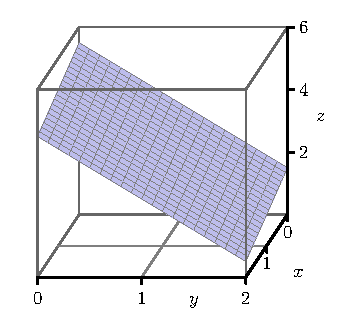
\includegraphics{figures/fig_10_4_tangent_8.eps}
      \hspace*{20pt}
      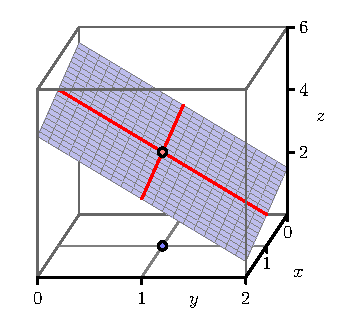
\includegraphics{figures/fig_10_4_tangent_7.eps}
    \end{center}
    \caption{The graph of $f(x,y)=3-\frac12(x-1)-2(y-1)$.}
    \label{F:10.4.tangent.7}
  \end{figure}

  \ba
  \item If $(x_0,y_0)=(1,1)$, what are the coordinates of the point on
    the plane above $(x_0,y_0)$?  How is this quantity reflected in
    the expression $z=z_0 + a(x-x_0) + b(y-y_0)$?

  \item Write the function $f(x, y_0) = f(x,1)$ that describes the
    trace of $f(x,y)$ with $y=y_0=1$.  Sketch its graph on the left of
    Figure \ref{F:10.4.preview.1}.  What is the slope of this trace?
    How is this slope related to the partial derivatives of $f$?  How
    does this slope appear in the expression $z=z_0 + a(x-x_0) +
    b(y-y_0)$? 

  \begin{figure}[ht]
    \begin{center}
      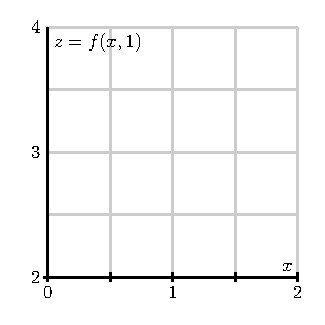
\includegraphics{figures/fig_10_4_preview_1.eps}
      \hspace*{20pt}
      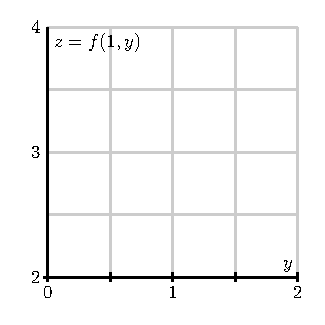
\includegraphics{figures/fig_10_4_preview_2.eps}
    \end{center}
    \caption{The traces of $f(x,y)=3-\frac12(x-1)-2(y-1)$.}
    \label{F:10.4.preview.1}
  \end{figure}

  \item Similarly, write the function $f(x_0, y) = f(1,y)$ that describes the
    trace of $f(x,y)$ with $x=x_0=1$.  Sketch its graph on the right of
    Figure \ref{F:10.4.preview.1}.  What is the slope of this trace?
    How is this slope related to the partial derivatives of $f$?  How
    does this slope appear in the expression $z=z_0 + a(x-x_0) +
    b(y-y_0)$? 

  \item If a plane is the graph of the function $z = f(x,y) = z_0 +
    a(x-x_0) + b(y-y_0)$, use the previous parts of this activity to
    explain why this may be written as 
    $$
    z = f(x_0, y_0) + f_x(x_0,y_0)(x-x_0) + f_y(x_0,y_0)(y-y_0).
    $$

  \ea



\end{pa} \afterpa 

\subsection*{The tangent plane}

%When we looked at the graph of a differentiable single-variable
%function on a small scale, we found that it looked like a line,
%which we called the tangent line.  


Before stating the formula for the equation of the tangent plane at a point for
a general function $f(x,y)$, we need to discuss a mild technical
condition.   As we have noted, when we look at the graph of a single-variable
function on a small scale near a point $x_0$, we expect to see a line;
in this case, we say that {\em $f$ is locally linear near $x_0$} since
the graph looks like a linear function locally around $x_0$.  Of
course, there are functions, such as $f(x)=|x|$, that are not locally
linear at every point.  In single-variable calculus, we learn that if the derivative of a function exists at a point, 
then the function is guaranteed to be locally linear there.

In a similar way, we say that a two-variable function {\em $f$ is
  locally linear\index{function!locally linear} near $(x_0,y_0)$} provided that the graph of $f$ looks like a
plane when viewed on a small scale near $(x_0,y_0)$.  There are, of
course, functions that are not locally linear at some points
$(x_0,y_0)$.  However, it turns out that if the first-order partial derivatives, $f_x$ and $f_y$, are continuous near
$(x_0,y_0)$, then $f$ is locally linear at $(x_0,y_0)$ and the graph
looks like a plane, which we call the tangent plane, when viewed on a
small scale.  Moreover, when a function is locally linear at a point, we will also say it is \emph{differentiable} at that point.

\vspace*{5pt}
\nin \framebox{\hspace*{3 pt}
\parbox{6.25 in}{If $f$ is a function of the independent variables $x$ and $y$ and both $f_x$ and $f_y$ exist and are continuous in an open disk containing 
the point $(x_0,y_0)$, then $f$ is \textbf{differentiable}\index{function!differentiable} at $(x_0,y_0)$.
} \hspace*{3 pt}}
\vspace*{5pt}


So, whenever a function $z = f(x,y)$ is differentiable at a point $(x_0,y_0)$, it follows that the function has a tangent plane at $(x_0,y_0)$.  Viewed up close, the tangent plane and the function are then virtually indistinguishable.  In addition, as in Preview Activity~\ref{PA:10.4}, we find the following general formula for the tangent plane.

\vspace*{5pt}
\nin \framebox{\hspace*{3 pt}
\parbox{6.25 in}{
  If $f(x,y)$ has continuous first-order partial derivatives, 
  then the equation of the plane
    tangent to the graph of $f$ at the point $(x_0,y_0,f(x_0,y_0))$ is
  \begin{equation}
    z = f(x_0,y_0) + f_x(x_0,y_0)(x-x_0) + f_y(x_0,y_0)(y-y_0).
    \label{eq:10.4.tan_plane}
  \end{equation}
} \hspace*{3 pt}}
\vspace*{5pt}

Finally, one important note about the form of the equation for the tangent plane, $z = f(x_0,y_0) + f_x(x_0,y_0)(x-x_0) + f_y(x_0,y_0)(y-y_0)$.  Say, for example, that we have the particular tangent plane $z = 7 - 2(x-3) + 4(y+1)$.  Observe that we can immediately read from this form that  $f_x(3,-1) = -2$ and $f_y(3,-1) = 4$; furthermore, $f_x(3,-1)=-2$ is the slope of the trace to both $f$ and the tangent plane in the $x$-direction at $(-3,1)$.  In the same way, $f_y(3,-1) = 4$ is the slope of the trace of both $f$ and the tangent plane in the $y$-direction at $(3,-1)$.

\begin{activity} \label{A:10.4.1} Find the equation of the tangent plane to $f(x,y) = x^2y$ at the point $(1,2)$.


\end{activity}
\begin{smallhint}

\end{smallhint}
\begin{bighint}

\end{bighint}
\begin{activitySolution}
Since $\frac{\partial f}{\partial x} = 2xy$ and $\frac{\partial f}{\partial y} = x^2$ we have $f_x(1,2) = 4$ and $f_y(1,2) =1$. So the equation of the plane tangent to $f$ at $(1,2)$ is
\[z = f_x(1,2)(x-1) + f_y(1,2)(y-2) + f(1,2)\]
or
\[z = 4(x-1) + (y-2) + 2.\]
\end{activitySolution}
\aftera


\subsection*{Linearization}

In single variable calculus, an important use of the tangent line is
to approximate the value of a differentiable function.  Near the point $x_0$, the
tangent line to the graph of $f$ at $x_0$ is close to the
graph of $f$ near $x_0$, as shown in Figure \ref{F:10.4.2d.linear}.

\begin{figure}[ht]
  \begin{center}
    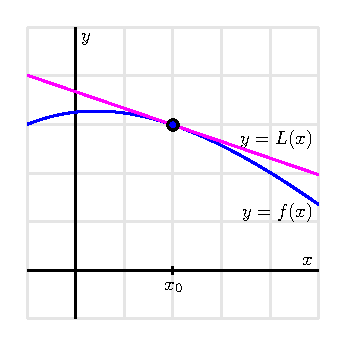
\includegraphics{figures/fig_10_4_2d_linear.eps}
    \hspace*{20pt}
    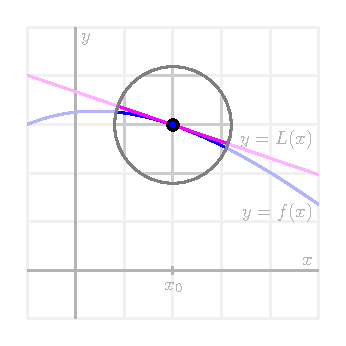
\includegraphics{figures/fig_10_4_2d_linear_gray.eps}
  \end{center}
  \caption{The linearization of the single-variable function $f(x)$.}
  \label{F:10.4.2d.linear}
\end{figure}

In this single-variable setting, we let $L$ denote the function whose graph is the tangent line, and thus
$$
L(x) = f(x_0) + f'(x_0)(x-x_0)
$$
Furthermore, observe that $f(x) \approx L(x)$ near $x_0$.  We call $L$ the
{\em linearization} of $f$.

In the same way, the tangent plane to the graph of a differentiable function $z = f(x,y)$ at a point
$(x_0,y_0)$ provides a good approximation of $f(x,y)$ near $(x_0,
y_0)$.  Here, we define the linearization, $L$, to be the two-variable function whose
graph is the tangent plane, and thus
$$
L(x,y) = f(x_0,y_0) + f_x(x_0,y_0)(x-x_0) +
f_y(x_0,y_0)(y-y_0).
$$
Finally, note that $f(x,y)\approx L(x,y)$ for points near $(x_0,
y_0)$. This is illustrated in Figure \ref{F:10.4.tangent.9}.

\begin{figure}[ht]
  \begin{center}
    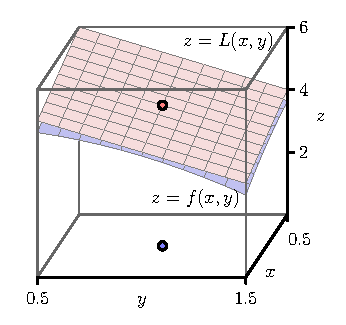
\includegraphics{figures/fig_10_4_tangent_9.eps}
  \end{center}
  \caption{The linearization of $f(x,y)$.}
  \label{F:10.4.tangent.9}
\end{figure}

\begin{activity} \label{A:10.4.11} In what follows, we find the linearization of several different functions that are given in algebraic, tabular, or graphical form.
\ba

\item Find the linearization $L(x,y)$ for the function $g$ defined by 
$$
g(x,y) = \frac{x}{x^2+y^2}
$$
at the point $(1,2)$.  Then use the linearization to estimate the value of
 $g(0.8, 2.3)$.

\item Table \ref{T:10.4.wind.chill} provides a collection of
  values of the wind chill $w(v,T)$, in degrees Fahrenheit, as a
  function of  wind speed, in miles per hour, and temperature, also in degrees Fahrenheit.
 

\begin{table}[ht] 
  \begin{center}
    \begin{tabular}{|c||c|c|c|c|c|c|c|c|c|c|c|}
      \hline
      $v \backslash T$  
         &-30  &-25 &-20 &-15 &-10 &-5  &0   &5   &10  &15  &20  \\
      \hhline{|=|=|=|=|=|=|=|=|=|=|=|=|}
      5  &-46	&-40 &-34 &-28 &-22 &-16 &-11 &-5 &1 &7 &13  \\
      \hline
      10 &-53	&-47 &-41 &-35 &-28 &-22 &-16 &-10 &-4 &3 &9   \\
      \hline
      15 &-58	&-51 &-45 &-39 &-32 &-26 &-19 &-13 &-7 &0 &6  \\
      \hline
      20 &-61	&-55 &-48 &-42 &-35 &-29 &-22 &-15 &-9 &-2 &4  \\
      \hline
      25 &-64	&-58 &-51 &-44 &-37 &-31 &-24 &-17 &-11 &-4 &3 \\
      \hline
      30 &-67	&-60 &-53 &-46 &-39 &-33 &-26 &-19 &-12 &-5 &1 \\
      \hline
      35 &-69	&-62 &-55 &-48 &-41 &-34 &-27 &-21 &-14 &-7 &0 \\
      \hline
      40 &-71	&-64 &-57 &-50 &-43 &-36 &-29 &-22 &-15 &-8 &-1 \\
      \hline
    \end{tabular}
    \caption{Wind chill as a function of wind speed and temperature.}
    \label{T:10.4.wind.chill}
  \end{center}
\end{table}
%\begin{table}[ht]
%  \begin{center}
%    \begin{tabular}{|c||c|c|c|c|c|c|c|c|c|c|c|}
%      \hline
%      $v \backslash T$  
%         &-30  &-25 &-20 &-15 &-10 &-5  &0   &5   &10  &15  &20  \\
%      \hhline{|=|=|=|=|=|=|=|=|=|=|=|=|}
%      5  &-35  &-31 &-26 &-20 &-15 &-11 &-6  &1   &7   &12  &16  \\
%      \hline
%      10 &-58  &-52 &-45 &-38 &-31 &-27 &-22 &-15 &-9  &-2  &2   \\
%      \hline
%      15 &-70  &-65 &-60 &-51 &-45 &-40 &-33 &-25 &-18 &-11 &-6  \\
%      \hline
%      20 &-81  &-76 &-68 &-60 &-52 &-46 &-40 &-32 &-24 &-17 &-9  \\
%      \hline
%      25 &-89  &-83 &-75 &-67 &-58 &-52 &-45 &-37 &-29 &-22 &-15 \\
%      \hline
%      30 &-94  &-87 &-78 &-70 &-63 &-56 &-49 &-41 &-33 &-26 &-18 \\
%      \hline
%      35 &-98  &-90 &-83 &-72 &-67 &-60 &-52 &-43 &-35 &-27 &-20 \\
%      \hline
%      40 &-101 &-94 &-87 &-76 &-69 &-62 &-54 &-45 &-36 &-29 &-22 \\
%      \hline
%    \end{tabular}
%    \caption{Wind chill as a function of temperature and wind speed}
%    \label{T:10.2.wind.chill}
%  \end{center}
%\end{table}


Use the data to first estimate the appropriate partial derivatives, and then find the linearization $L(v,T)$ at the point $(25,-10)$.  Finally, use the linearization to estimate $w(25,-12)$, $w(23,-10)$, and $w(23,-12)$.

\item Figure \ref{F:10.4.activity.contour} gives a contour
  plot of a differentiable function $f$.  

  \begin{figure}[ht]
    \begin{center}
      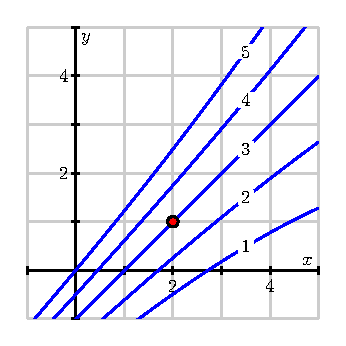
\includegraphics{figures/fig_10_3_activity_contour.eps}
    \end{center}
    \caption{A contour plot of $f(x,y)$.}
    \label{F:10.4.activity.contour}
  \end{figure}

  After estimating appropriate partial derivatives, determine the linearization $L(x,y)$ at the point $(2,1)$, and use it to
  estimate $f(2.2, 1)$, $f(2, 0.8)$, and $f(2.2, 0.8)$.



\ea

\end{activity}

\begin{activitySolution}
\ba
\item To find the linearization of $g$ we need the first order partials. Now
\begin{align*}
g_x(x,y) &= \frac{(x^2+y^2)-2x^2}{(x^2+y^2)^2} = \frac{y^2-x^2}{(x_2+y^2)^2} \\
g_y(x,y) &= \frac{-2xy}{(x^2+y^2)^2}.
\end{align*}
So the linearization of $g$ at the point (1,2) is
\[L(x,y) = g(1,2) +g_x(1,2)(x-1) + g_y(1,2)(y-2) = \frac{1}{5} + \frac{3}{25}(x-1) - \frac{4}{25}(y-2).\]
It follows that 
\[g(0.8,2.3) \approx L(0.8,2.3) = \frac{1}{5} - \frac{3}{25}(0.2) - \frac{4}{25}(0.3) = 0.128.\]
Since $g(0.8,2.3) \approx 0.135$, we have a fair approximation. This should be expected since the step sizes of 0.2 and 0.3 are not that small. 
\item We need $w_v(25,-10)$ and $w_T(25,-10)$ to find the linearization. Using the symmetric difference quotients gives us
\begin{align*}
w_v(25,-10) &\approx \frac{w(30,-10)-w(20,-10)}{10} = \frac{-39-(-35)}{10} = -0.4 \\
w_T(25,-10) &\approx \frac{w(25,-5)-w(25,-15)}{10} = \frac{-31-(-44)}{10} = 0.7.
\end{align*}  
So the linearization of $w$ at $(25, -10)$ is 
\[L(v,T) \approx -37 - 0.4(v-25) + 0.7(T+10).\]
Thus,
\begin{align*}
w(25,-12) &\approx L(25,-12) \approx -37 - 0.4(0) + 0.7(-2) = -38.4 \\
w(23, -10) &\approx L(23,-10) \approx -37 - 0.4(-2) + 0.7(0) = -36.2 \\
w(23, -12) &\approx L(23,-12) \approx -37 - 0.4(-2) + 0.7(-2) = -37.6.
\end{align*}

\item We need $f_x(2,1)$ and $f_y(2,1)$ to find the linearization. Using the symmetric difference quotients gives us
\begin{align*}
f_x(2,1) &\approx \frac{f(3,1)-f(1,1)}{2} \approx \frac{1.9-4.8)}{2} = -1.45 \\
f_y(2,1) &\approx \frac{f(2,2)-f(2,0)}{2} \approx \frac{4.3-1.8}{10} = 1.25.
\end{align*}  
So the linearization of $f$ at $(2, 1)$ is 
\[L(x,y) \approx 3 - 1.45(x-2) + 1.25(y-1).\]
Thus,
\begin{align*}
f(2.2,1) &\approx L(2.2,1) \approx 3 - 1.45(0.2) + 1.25(0) = 2.71 \\
f(2, 0.8) &\approx L(2, 0.8) \approx 3 - 1.45(0) + 1.25(-0.2) = 2.75 \\
f(-1.8, 2.1) &\approx L(2.2, 0.8) \approx 3 - 1.45(0.2) + 1.25(-0.2) = 2.46.
\end{align*}
The last two should be poor approximations since we are approximating quite far from the base point of $(2,1)$.
\ea
\end{activitySolution}

\aftera


\subsection*{Differentials}

As we have seen, the linearization $L(x,y)$ enables us to estimate the value of $f(x,y)$ for points $(x,y)$ near the base point
$(x_0, y_0)$. 
Sometimes, however, we are more interested in the {\em change} in the
function $f(x,y)$ as we move from the base point $(x_0,y_0)$ to another
point $(x,y)$.  

\begin{figure}[ht]
  \begin{center}
    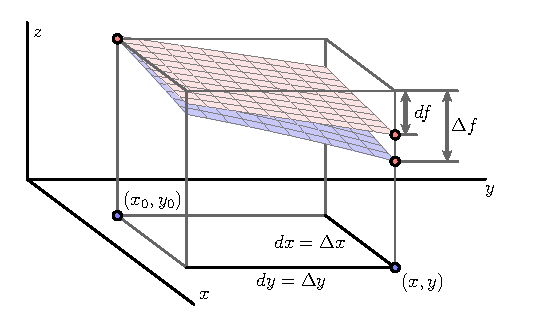
\includegraphics{figures/fig_10_4_tangent_10.eps}
  \end{center}
  \caption{The differential $df$ measures the approximate change in
    $f(x,y)$.} 
  \label{F:10.4.differential}
\end{figure}

Figure \ref{F:10.4.differential} illustrates this situation.  Suppose
we are at the point $(x_0,y_0)$, and we know the value $f(x_0,y_0)$ of $f$ at $(x_0,y_0)$.  If we consider the displacement $\langle \Delta x, \Delta
y\rangle$ to a new point $(x,y) = (x_0+\Delta x, y_0
+ \Delta y)$, we would like to know how much the function has changed.
We denote this change by $\Delta f$, where
$$
\Delta f = f(x,y) - f(x_0, y_0).
$$
A simple way to estimate the change $\Delta f$ is to approximate it by
$df$, which represents the change in the linearization $L(x,y)$ as we move from
$(x_0,y_0)$ to $(x,y)$.  This gives
\begin{align*}
  \Delta f \approx df &= L(x,y)-f(x_0, y_0)  \\
  &= [f(x_0,y_0)+ f_x(x_0,y_0)(x-x_0) +
  f_y(x_0,y_0)(y-y_0)] - f(x_0, y_0) \\
  &= f_x(x_0,y_0)\Delta x + f_y(x_0, y_0)\Delta y. 
\end{align*}
%This leaves us with $\Delta f \approx df = f_x(x_0,y_0)\Delta x +
%f_y(x_0, y_0)\Delta y$.  
For consistency, we will denote the
change in the independent variables as $dx = \Delta x$ and $dy =
\Delta y$, and thus
\begin{equation}
  \Delta f \approx df = f_x(x_0,y_0)~dx + f_y(x_0,y_0)~dy.
  \label{E:10.4.differential}
\end{equation}
Expressed equivalently in Leibniz notation, we have
\begin{equation}
  df = \frac{\partial f}{\partial x}~dx + \frac{\partial f}{\partial
    y}~dy.
  \label{E:10.4.differential.leib}
\end{equation}


We call the quantities $dx$, $dy$, and $df$ {\em differentials}, and
we think of them as measuring small changes in the quantities $x$,
$y$, and $f$.  Equations (\ref{E:10.4.differential}) 
and (\ref{E:10.4.differential.leib}) express the
relationship between these changes.  Equation
(\ref{E:10.4.differential.leib}) resembles an important idea 
from single-variable calculus:  when $y$ depends on $x$,
it follows in the notation of differentials that 
$$
dy = y'~dx = \frac{dy}{dx}~dx.
$$

We will illustrate the use of differentials with an
example.  Suppose we have a machine that manufactures rectangles of
width $x=20$ cm and height $y=10$ cm.  However, the machine isn't
perfect, and therefore the width could be off by $dx = \Delta x = 0.2$ cm and
the height could be off by $dy = \Delta y = 0.4$ cm.  

The area of the rectangle is 
$$
A(x,y) = xy,
$$
so that the area of a perfectly manufactured rectangle is $A(20, 10) =
200$ square centimeters.  Since the machine isn't perfect, we would
like to know how much the area of a given manufactured rectangle could differ from the
perfect rectangle.  We will estimate the uncertainty in the area using
(\ref{E:10.4.differential}), and find that
$$
\Delta A \approx dA = A_x(20, 10)~dx + A_y(20,10)~dy.
$$
Since $A_x = y$ and $A_y = x$, we have
$$
\Delta A \approx dA = 10~dx + 20~dy = 10\cdot0.2 + 20\cdot0.4 = 10.
$$
That is, we estimate that the area in our rectangles could be off by
as much as 10 square centimeters.

\begin{activity} \label{A:10.4.12} The questions in this activity explore the differential in several different contexts.
\ba
\item Suppose that the elevation of a landscape is given by the
  function $h$, where we additionally know that $h(3,1) = 4.35$, $h_x(3,1) = 0.27$, and $h_y(3,1) = -0.19$.  Assume that $x$ and $y$ are measured in miles in the easterly and northerly directions, respectively, from some base point $(0,0)$.

  Your GPS device says that you are currently at the point $(3,1)$.
  However, you know that the coordinates are only accurate to within
  $0.2$ units; that is, $dx = \Delta x = 0.2$ and $dy= \Delta y =
  0.2$.  Estimate the uncertainty in your elevation using differentials.

\item The pressure, volume, and temperature of an ideal gas are
  related by the equation 
  $$
  P= P(T,V) = 8.31 T/V,
  $$
  where $P$ is measured in kilopascals, $V$ in liters, and $T$ in
  kelvin.  Find the pressure when the volume is 12 liters and the
  temperature is 310 K.  Use differentials to estimate the change
  in the pressure when the volume increases to 12.3 liters and the
  temperature decreases to 305 K.

\item Refer to Table \ref{T:10.4.wind.chill}, the table of
  values of the wind chill $w(v,T)$, in degrees Fahrenheit, as a
  function of temperature, also in degrees Fahrenheit, and 
  wind speed, in miles per hour.  
  
  Suppose your anemometer says the wind is blowing at $25$ miles per hour and your thermometer shows a reading of $-15^\circ$ degrees.
  However, you know your thermometer is only accurate to within
  $2^\circ$ degrees and your anemometer is only accurate to within $3$
  miles per hour.  What is the wind chill based on your measurements?
  Estimate the uncertainty in your measurement of the wind chill.

\ea

\end{activity}

\begin{activitySolution}
\ba
\item The error is approximated by the differential 
\[\Delta h \approx dh = h_x(3,1)~dx + h_y(3,1)~dy = 0.27(0.2) - 0.19(0.2) = 0.016.\]

\item First note that $P(310,12) = 214.675$. To find the differential, we need both $P_T(310,12)$ and $P_V(310,12)$. Our differentiation rules give us 
\begin{align*}
P_T(T,V) &= 8.31\frac{1}{V} \\
P_V(T,V) &= -8.31\frac{T}{V^2}.
\end{align*}
So $P_T(310,12) = 0.6925$ and $P_V(310,12) \approx -17.8896$. We have $dT = -5$ and $dV = 0.3$, and the change in pressure is 
\[\Delta P \approx dP = P_T(310,12)~dT + P_V(310,12)~dV \approx 0.6925(-5) - 17.8896(0.3) = -8.82938.\]
Therefore, the pressure decreases by about 8.82938 kilopascals.

\item First note that 
\begin{align*}
w_v(25,-15) &\approx \frac{w(30,-15)-w(20,-15)}{10} = \frac{-46-(-42)}{10} = -0.4 \\
w_T(25,-15) &\approx \frac{w(25,-10)-w(25,-20)}{10} = \frac{-37-(-51)}{10} = 1.4.
\end{align*}
The wind chill is $w(25,-15) = -44^{\circ}F$. But since $dT = 2$ and $dv = 3$, our wind chill measurement has an error of
\[\Delta w \approx dw = -0.4(3) + 1.4(2) = 1.6^{\circ}F.\]


\ea
\end{activitySolution}

\aftera




\begin{summary}
\item A function $f$ of two independent variables is locally linear at
  a point $(x_0,y_0)$ if the graph of $f$ looks like a plane 
  as we zoom in on the graph around the point $(x_0,y_0)$.  In this
  case, the equation of the tangent plane is given by
  $$
  z = f(x_0,y_0) + f_x(x_0,y_0)(x-x_0) + f_y(x_0,y_0)(y-y_0).
  $$
\item The tangent plane $L(x,y) = f(x_0,y_0) + f_x(x_0,y_0)(x-x_0) + f_y(x_0,y_0)(y-y_0)$, when considered as a function, is
  called the linearization of a differentiable function $f$ at $(x_0,y_0)$ and may be used
  to estimate values of $f(x,y)$;  that is, $f(x,y) \approx L(x,y)$
  for points $(x,y)$ near $(x_0,y_0)$.
  
\item A function $f$ of two independent variables is differentiable at $(x_0,y_0)$ provided that both $f_x$ and $f_y$ exist and are continuous in an open disk containing 
the point $(x_0,y_0)$.

\item The differential $df$ of a function $f(x,y)$ is related to the
  differentials $dx$ and $dy$ by
  \[df = f_x(x_0,y_0) dx + f_y(x_0,y_0)dy.\] 
  We can use this relationship to
  approximate small changes in $f$ that result from small changes in
  $x$ and $y$.
\end{summary}


\nin \hrulefill

\begin{exercises} 

\item \label{Ez:10.4.0}   Let $f$ be the function defined by $f(x,y) = x^{1/3}y^{1/3}$, whose graph is shown in Figure \ref{F:10.4.Not_diff}.
\begin{figure}[h]
\begin{center}
%\resizebox{!}{2.5in}{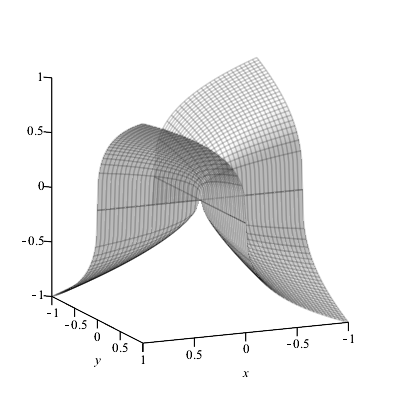
\includegraphics[trim=0cm 0.25cm 0.1cm 1.5cm,clip]{figures/10_4_Not_diff}}
  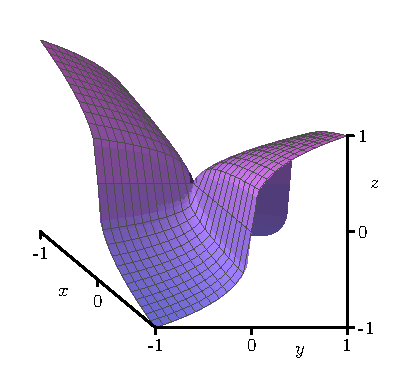
\includegraphics{figures/fig_10_4_not_diff.eps}
\end{center}
\caption{The surface for $f(x,y) = x^{1/3}y^{1/3}$.}
\label{F:10.4.Not_diff}
\end{figure}
    \ba
    \item Determine
    \[\lim_{h \to 0} \frac{f(0+h,0)-f(0,0)}{h}.\]
    What does this limit tell us about $f_x(0,0)$?

    \item Note that $f(x,y)=f(y,x)$, and this symmetry implies that $f_x(0,0) = f_y(0,0)$. So both partial derivatives of $f$ exist at $(0,0)$. A picture of the surface defined by $f$ near $(0,0)$ is shown in Figure \ref{F:10.4.Not_diff}. Based on this picture, do you think $f$ is locally linear at $(0,0)$? Why?

%crop graphics in animate trim=<left> <bottom> <right> <top> (add clip with \includegraphics)

    \item Show that the curve where $x=y$ on the surface defined by $f$ is not differentiable at 0. What does this tell us about the local linearity of $f$ at $(0,0)$?

    \item Is the function $f$ defined by $f(x,y) = \frac{x^2}{y^2+1}$ locally linear at $(0,0)$? Why or why not?

    \ea

\begin{exerciseSolution}
    \ba
    \item With $f(x,y) = x^{1/3}y^{1/3}$ we have 
    \[f_x(0,0) = \lim_{h \to 0} \frac{f(0+h,0)-f(0,0)}{h} = \lim_{h \to 0} \frac{(h^{1/3})(0)-0}{h} = 0.\]

    \item The graph of $f$ seems to indicate some kind of sharp fold in the surface around the point $(0,0)$, so it appears that $f$ is not locally linear at $(0,0)$.

    \item Wen $x=y$ $f$ has the form $f(x,x) = x^{2/3}$. Now
\[\frac{d f(x,x)}{dx}\biggm|_{x=0} = \lim_{h \to 0} \frac{(0+h)^{2/3} - 0}{h} = \lim_{h \to 0} \frac{h^{2/3}}{h} = \lim_{h \to 0} \frac{1}{h^{1/3}}\]
is undefined. Since $f$ does not have a derivative at $(0,0)$ along the path $y=x$, it follows that $f$ defined by $f(x,y) = x^{1/3}y^{1/3}$ is not locally linear at $(0,0)$. Note that neither $f_x$ nor $f_y$ is continuous at $(0,0)$.

    \item For $f(x,y) = \frac{x^2}{y^2+1}$ we have 
\[f_x(x,y) = \frac{2x(y^2+1)}{(y^2+1)^2} \ \text{ and } \ f_y(x,y) = \frac{-2x^2y}{(y^2+1)^2},\]
both of which are continuous around $(0,0)$. So $f$ is locally linear at $(0,0)$. 

    \ea
\end{exerciseSolution}

\item \label{Ez:10.4.1}   Let $g$ be a function that is differentiable at $(-2,5)$ and suppose that its tangent plane at this point is given by $z = -7 + 4(x+2) - 3(y-5)$.				
    \ba
   	\item Determine the values of $g(-2,5)$, $g_x(-2,5)$, and $g_y(-2,5)$.  Write one sentence to explain your thinking.
	\item Estimate the value of $g(-1.8, 4.7)$.  Clearly show your work and thinking.
	\item Given changes of $dx = -0.34$ and $dy = 0.21$, estimate the corresponding change in $g$ that is given by its differential, $dg$.
	\item Suppose that another function $h$ is also differentiable at $(-2,5)$, but that its tangent plane at $(-2,5)$ is given by $3x + 2y - 4z = 9.$  Determine the values of $h(-2,5)$, $h_x(-2,5)$, and $h_y(-2,5)$, and then estimate the value of $h(-1.8, 4.7)$.  Clearly show your work and thinking.
    \ea

\begin{exerciseSolution}
    \ba
   	\item Since the equation of the plane tangent to $g$ at $(-2,5)$ is 
\[L(x,y) = g(-2,5) + g_2(-2,5)(x+2) + g_y(-2,5)(y-5) = -7 + 4(x+2) - 3(y-5)\]
we see that  
\[g(-2,5) = -7, \ g_x(-2,5) = 4, \ \text{ and } \ g_y(-2,5) = -3.\]
	\item The tangent plane approximates the graph of the surface near the point of tangency, so
\[L(x,y) = -7 + 4(x+2) - 3(y-5) \approx g(x,y)\]
when $(x,y)$ is close to $(-2,5)$. Thus,
\[g(-1.8,4.7) \approx L(-1.8,4.7) = -7 + 4(-0.2) - 3(-0.3) = -6.9.\]
	\item The differential $dg$ has the form 
\[dg = g_x(x_0, y_0)dx + g_y(x_0, y_0)dy.\]
In this case, $(x_0, y_0) = (-2,5)$, $dx = -0.34$, and $dy = 0.21$, so
\[dg = 4(-0.34) - 3(0.21) = -1.99.\]
	\item Since the tangent plane $z = \frac{1}{4}(3x+2y-9)$ to $h$ at $(-2,5)$ intersects the graph of $h$ at $(-2,5)$, it follows that $h(-2,5) = \frac{1}{4}(3(-2)+2(5)-9) = -\frac{5}{4} = -1.25$. We also have $h_x(-2,5) = 3$ and $h_y(-2,5) = 2$. Then
\[h(-1.8, 4.7) \approx \frac{1}{4}(3(-1.8)+2(5)-9) = -1.1.\]

    \ea
\end{exerciseSolution}

\item \label{Ez:10.4.2}   In the following questions, we determine and apply the linearization for several different functions.				
    \ba
   	\item Find the linearization $L(x,y)$ for the function $f$ defined by $f(x,y) = \cos(x)(2e^{2y}+e^{-2y})$
at the point $(x_0,y_0) = (0,0)$.  Hence use the linearization to estimate
the value of $f(0.1, 0.2)$.  Compare your estimate to the actual value of $f(0.1, 0.2)$.

	\item The Heat Index, $I$, (measured in apparent degrees F) is a function of the actual temperature $T$ outside (in degrees F) and the relative humidity $H$ (measured as a percentage).  A portion of the table which gives values for this function, $I(T,H)$, is provided below:
\begin{center}
\begin{tabular}{|l||r|r|r|r|} \hline
\emph{T} $\downarrow \backslash$ \emph{H} $\rightarrow$ & 70 &	75 & 80 &	85  \\ \hhline{|=|=|=|=|=|}
90 & 106 & 109 & 112 & 115  \\ \hline
92 & 112 & 115 & 119 & 123  \\ \hline
94 & 118 & 122 & 127 & 132  \\ \hline
96 & 125 & 130 & 135 & 141  \\ \hline
\end{tabular}
\end{center}
Suppose you are given that $I_T(94,75) = 3.75$ and $I_H(94,75) = 0.9$.  Use this given information and one other value from the table to estimate the value of $I(93.1,77)$ using the linearization at $(94,75)$.  Using proper terminology and notation, explain your work and thinking.
	\item Just as we can find a local linearization for a differentiable function of two variables, we can do so for functions of three or more variables.  By extending the concept of the local linearization from two to three variables, find the linearization of the function $h(x,y,z) =
  e^{2x}(y+z^2)$ at the point $(x_0,y_0,z_0) = (0, 1, -2)$.  Then, use the
  linearization to estimate the value of $h(-0.1, 0.9, -1.8)$.
    \ea

\begin{exerciseSolution}
    \ba
   	\item If $f(x,y) = \cos(x)(2e^{2y}+e^{-2y})$, then
\[f_x(x,y) = -\sin(x)(2e^{2y}+e^{-2y}) \ \text{ and } \ f_y(x,y) = \cos(x)\left(4e^{2y} - 2e^{-2y}\right).\]
So
\[f_x(0,0) = 0 \ \text{ and } \ f_y(0,0) = 2.\]
So the linearization of $f$ at $(0,0)$ is 
\[L(x,y) = f(0,0) + f_x(0,0)(x-0)+f_y(0,0)(y-0) = 3+2y.\]
Then
\[f(0.1,0.2) \approx L(0.1,0.2) = 3.4.\]
By calculator, the value of $f(0.1,0.2)$ is approximately $3.635714815$, so our approximation with the linearization is off by about $0.23$.

	\item Since $I(94,75) = 122$, the linearization of $I$ at $(94,75)$ is 
\[L(x,y) = I(94,75) + I_T(94,75)(T-94) + I_H(94,75)(H-75) = 122 + 3.75(T-94) + 0.9(H-75).\]
Thus,
\[I(93.1,77) \approx L(93.1,77) = 122 + 3.75(-0.9) + 0.9(2) = 120.425.\]

	\item The linearization of $h$ at $(x_0,y_0,z_0)$ will be 
\[L(x,y,z) = h(x_0,y_0,z_0) + h_x(x_0,y_0,z_0)(x-x_0) + h_y(x_0,y_0,z_0)(y-y_0) + h_z(x_0,y_0,z_0)(z-z_0).\]
For our function $h$ we have 
\[h_x(x,y,z) = 2e^{2x}(y+z^2), \ h_y(x,y,z) = e^{2x}, \ \text{ and } \ h_z(x,y,z) = e^{2x}(2z).\]
So
\[h_x(0,1,-2) = 10, \ h_y(0,1,-2) = 1, \ \text{ and } \ h_z(0,1,-2) = -4\]
and the linearization of $h$ at $(0,1,-2)$ is 
\[L(x,y,z) = 5 + 10x + (y-1) - 4(z+2).\]
Thus,
\[h(-0.1, 0.9, -1.8) \approx L(-0.1, 0.9, -1.8) = 3.1.\]
	\ea
	
\end{exerciseSolution}

\item \label{Ez:10.4.3}   In the following questions, we investigate two different applied settings using the differential.

\ba

	\item Let $f$ represent the vertical displacement in centimeters from the rest position of a string (like a guitar string) as a function of the distance $x$ in centimeters from the fixed left end of the string and $y$ the time in seconds after the string has been plucked.\footnote{An interesting video of this can be seen at \url{https://www.youtube.com/watch?v=TKF6nFzpHBUA}.} A simple model for $f$ could be
\[f(x,y) = \cos(x)\sin(2y).\]
Use the differential to approximate how much more this vibrating string is vertically displaced from its position at $(a,b) = \left(\frac{\pi}{4}, \frac{\pi}{3} \right)$ if we decrease $a$ by $0.01$ cm and increase the time by $0.1$ seconds. Compare to the value of $f$ at the point $\left(\frac{\pi}{4}-0.01, \frac{\pi}{3}+0.1\right)$.

   	\item Resistors used in electrical circuits have colored bands painted
  on them to indicate the amount of resistance and the possible error
  in the resistance.  When three resistors, whose resistances are
  $R_1$, $R_2$, and $R_3$, are connected in parallel, the total
  resistance $R$ is given by
  $$
  \frac1R = \frac1{R_1} + \frac1{R_2} + \frac1{R_3}.
  $$
  Suppose that the resistances are $R_1=25\Omega$, $R_2=40\Omega$, and
  $R_3=50\Omega$.  Find the total resistance $R$.

  If you know each of $R_1$, $R_2$, and $R_3$ with a possible error of
  $0.5$\%, estimate the maximum error in your calculation of $R$.

\ea

\begin{exerciseSolution}
\ba
\item First note that
\[\frac{\partial f}{\partial x} = -\sin(x)\sin(2y) \ \ \text{ and } \ \ \frac{\partial f}{\partial y} = 2\cos(x)\cos(2y)\]
and
\[f_x\left(\frac{\pi}{4}, \frac{\pi}{3}\right) = -\sin\left(\frac{\pi}{4}\right)\sin\left(\frac{2\pi}{3}\right) = -\frac{\sqrt{6}}{4} \ \ \text{ and } \ \ f_y\left(\frac{\pi}{4}, \frac{\pi}{3}\right) = 2\cos\left(\frac{\pi}{4}\right)\cos\left(\frac{2\pi}{3}\right) = -\frac{\sqrt{2}}{2}.\]

So with $dx = -0.01$ and $dy = 0.1$ we have 
\[df = f_x(a,b)(-0.01) + f_y(a,b)(y-b) = -\frac{\sqrt{6}}{4}(-0.01) - \frac{\sqrt{2}}{2}(0.1) \approx -0.065.\]
So the string is vertically displaced approximately $-0.064$ centimeters from its position at $(a,b)$. Comparing to the exact displacement
\[f(a,b) - f(a-0.01, b+0.1) \approx 0.077,\]
we see that our approximation is off by about $0.01$.

\item The total resistance $R$ satisfies 
\[\frac{1}{R} = \frac{1}{25} + \frac{1}{40} + \frac{1}{50} = \frac{17}{200},\]
so 
\[R = \frac{200}{17}.\]
We can write $R$ as 
\[R = \frac{R_1R_2R_3}{R_2R_3+R_1R_3+R_1R_2}.\]
Then
\begin{align*}
R_{R_1}(R_1,R_2,R_3) &= \frac{(R_2R_3+R_1R_3+R_1R_2)(R_2R_3)-R_1R_2R_3(R_3+R_2)}{(R_2R_3+R_1R_3+R_1R_2)^2} \\
R_{R_2}(R_1,R_2,R_3) &= \frac{(R_2R_3+R_1R_3+R_1R_2)(R_1R_3)-R_1R_2R_3(R_3+R_1)}{(R_2R_3+R_1R_3+R_1R_2)^2} \\
R_{R_3}(R_1,R_2,R_3) &= \frac{(R_2R_3+R_1R_3+R_1R_2)(R_1R_2)-R_1R_2R_3(R_2+R_1)}{(R_2R_3+R_1R_3+R_1R_2)^2}.
\end{align*}
This gives us
\begin{align*}
R_{R_1}(25, 40, 50) &= \frac{64}{289} \\
R_{R_2}(25, 40, 50) &= \frac{25}{289}  \\
R_{R_3}(25, 40, 50) &= \frac{16}{289}.
\end{align*}
If $dR_1 = dR_2 = dR_3 = 0.005$, then 
\begin{align*}
dR &= R_{R_1}(25, 40, 50) dR_1 + R_{R_2}(25, 40, 50) dR_2 + R_{R_3}(25, 40, 50) dR_3 \\
	&= \left(\frac{64}{289} + \frac{25}{289} + \frac{16}{289} \right) (0.005) \\
	&\approx 0.0018.
\end{align*}
So the maximum error in our calculation is about 0.18\%. 

\ea
\end{exerciseSolution}
\end{exercises}
\afterexercises


\clearpage
